%This work is licensed under the Creative Commons License Attribution 4.0 International (CC-BY 4.0) 
%https://creativecommons.org/licenses/by/4.0/legalcode 
\documentclass[rgb]{standalone}
\usepackage{tikz, pgfplots}
\begin{document}
	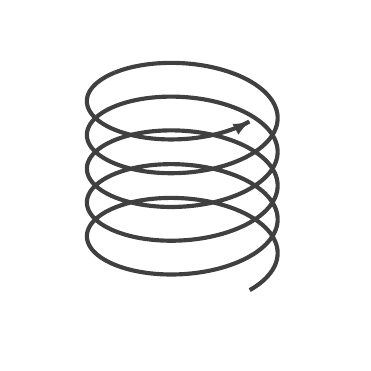
\begin{tikzpicture}[scale=0.5, font=\Large]
		\draw[draw=none] (-0.5,-0.5) -- (-0.5,7.5) -- (7.5,7.5) -- (7.5,-0.5) -- cycle;
		\begin{axis}[scale=1,clip=false,
		hide axis,
		view={45}{45},
		xmin=-2, xmax=2,
		ymin=-2, ymax=2, 
		zmin=0, zmax=5.5,
		]	
		\addplot3[line width=3pt,darkgray,variable=x,smooth,domain=0:9,samples = 500, samples y=0] ({2*cos(180*x)},{2*sin(180*x)}, {x});
		\addplot3[line width=3pt,darkgray,-latex,variable=x,smooth,domain=9:10,samples = 500, samples y=0] ({2*cos(180*x)},{2*sin(180*x)}, {x});
		\end{axis}
	\end{tikzpicture}
\end{document}